% ============================================================
%  The Geometry of Attention: From Burer-Monteiro Factorization
%  to Margin Rank Theory
%  IE210 Optimization Modelling ,  IIT Bombay ,  2026
% ============================================================
% \documentclass[12pt, a4paper]{article}

% \usepackage[margin=2.5cm]{geometry}
% \usepackage{amsmath, amssymb, amsthm}
% \usepackage{mathtools}
% \usepackage{graphicx}
% \usepackage{booktabs}
% \usepackage{hyperref}
% \usepackage{xcolor}
% \usepackage{enumitem}

% \usepackage{float}
% \usepackage{caption}
% \usepackage{subcaption}
% \usepackage{algorithm}
% \usepackage{algpseudocode}
% \usepackage{fancyhdr}
% \usepackage{tikz}
% \usepackage{pgfplots}
% \pgfplotsset{compat=1.18}
% \usetikzlibrary{arrows.meta, positioning}

% % , , , - theorem environments , , , -
% \theoremstyle{plain}
% \newtheorem{theorem}{Theorem}[section]
% \newtheorem{lemma}[theorem]{Lemma}
% \newtheorem{corollary}[theorem]{Corollary}
% \newtheorem{proposition}[theorem]{Proposition}
% \theoremstyle{definition}
% \newtheorem{definition}[theorem]{Definition}
% \newtheorem{remark}[theorem]{Remark}
% \theoremstyle{remark}
% \newtheorem{conjecture}[theorem]{Conjecture}

% % , , , - math macros , , , -
% \newcommand{\R}{\mathbb{R}}
% \newcommand{\N}{\mathbb{N}}
% \newcommand{\E}{\mathbb{E}}
% \newcommand{\Sym}{\mathbb{S}}
% \newcommand{\norm}[1]{\left\lVert#1\right\rVert}
% \newcommand{\inner}[2]{\langle #1, #2 \rangle}
% \newcommand{\tr}{\operatorname{Tr}}
% \newcommand{\rank}{\operatorname{rank}}
% \newcommand{\Softmax}{\operatorname{Softmax}}
% \newcommand{\diag}{\operatorname{diag}}
% \DeclareMathOperator*{\argmin}{arg\,min}

% % , , , - header / footer , , , -
% \setlength{\headheight}{14pt}
% \pagestyle{fancy}
% \fancyhf{}
% \rhead{\small IE210 ,  IIT Bombay 2026}
% \lhead{\small The Geometry of Attention}
% \cfoot{\thepage}

% % ============================================================
% \begin{document}

% , , , - title page , , , -


% % ============================================================
% \section{Introduction}
% % ============================================================

% \subsection{Motivation}

% In modern Large Language Models (LLMs), the embedding dimension of each Transformer
% attention head ($d_{\text{head}}$) is almost universally set to 64 or 128. This number is
% not the product of mathematical analysis; it is chosen for memory-alignment efficiency on
% GPU hardware. The natural question, largely untouched by practitioners, is: \emph{How much
% of this capacity is actually used?}

% Formally, define the self-attention probability matrix for a sequence of $n$ tokens as
% \begin{equation}
%   A = \Softmax\!\left(\frac{QK^\top}{\sqrt{p}}\right), \quad Q, K \in \R^{n \times p},
%   \label{eq:attention}
% \end{equation}
% where $p = d_{\text{head}}$ is the projection dimension. Given a target attention matrix
% $M \in \R^{n \times n}$, what is the \emph{minimum} $p^*$ such that some $Q, K \in
% \R^{n\times p^*}$ satisfies $A = M$?

% This report documents our exploration of that question. The journey proceeded in three
% conceptual phases:
% \begin{enumerate}[label=\textbf{Phase \arabic*:}]
%   \item \textbf{Classical grounding.} We studied the Burer-Monteiro (BM) factorization for
%         Semidefinite Programs, verifying the Barvinok-Pataki bound and implicit
%         regularization in the symmetric setting.
%   \item \textbf{Extending to attention.} We modelled the Transformer attention head as an
%         asymmetric BM problem, discovered that the Pataki bound completely fails here,
%         and identified the Softmax Jacobian null space as the geometric reason.
%   \item \textbf{Margin Rank Theory.} We replaced the linear matrix-completion framework
%         with a margin-inequality framework, designed a Hard Bottleneck Predictor,
%         validated it on synthetic motifs, and applied it to GPT-2.
% \end{enumerate}

% \subsection{Research Contributions}
% \begin{itemize}
%   \item Empirical verification of the Barvinok-Pataki phase transition and implicit
%         regularization in the symmetric BM setting.
%   \item A clean ablation demonstrating the ``Geometric Warp Drive'' caused by the Softmax
%         operator.
%   \item A theoretical analysis of the Softmax Jacobian null space and its role in
%         converting constraint counts to margin inequalities.
%   \item The Margin Rank Theory and Hard Bottleneck Predictor algorithm.
%   \item Empirical validation on synthetic motifs and GPT-2, revealing 80--97\%
%         dimensional redundancy.
%   \item Architectural implications for heterogeneous Transformer design.
% \end{itemize}

% ============================================================
\section{Executive Summary}
% ============================================================

% The central finding of this work is that the standard $d_{\text{head}} = 64$ used in
% Transformer attention is dramatically oversized for most attention heads. The key chain of
% reasoning is as follows.

% Classical BM theory predicts that recovering an $n \times n$ matrix from $m$ linear
% equality constraints requires inner rank $p \geq \sqrt{2m}$ for optimization to be
% landscape-safe. For an $n \times n$ attention matrix with $m = n^2$ constraints, this gives
% $p \approx n\sqrt{2}$, well beyond the sequence length itself. Yet in practice, small
% $d_{\text{head}}$ values work empirically. This gap between theory and practice motivated
% our investigation.

% The resolution comes in two steps. First, the Softmax operator is not a passive
% nonlinearity, it actively absorbs $n$ row-sum constraints via its Jacobian null space,
% reducing the effective constraint count from $m = n^2$ to $m_{\text{eff}} = n(n-1)$.
% Second, even this corrected count over-predicts $p^*$, because the problem has shifted from
% linear algebra (exact equalities) to computational geometry (margin inequalities). The true
% structural capacity of an attention head is governed by its \emph{Margin Rank}: the minimum
% embedding dimension needed to geometrically separate target tokens from distractor tokens.

% Empirically, GPT-2 heads exhibit Margin Ranks of 1--5 out of an allocated $d_{\text{head}}
% = 64$, an 80--97\% redundancy. This motivates the design of Heterogeneous Transformers
% with dynamically allocated, head-specific embedding dimensions.


\section*{Executive Summary}

This project investigates the optimal dimensionality of transformation matrices (specifically $d_k$ and $d_v$) within Transformer architectures. The research evaluates theoretical optimization bounds, identifies their shortcomings in real-world application, and utilizes empirical observations and matrix sensing experiments to determine the true minimal required dimension ($p$) based on the target matrix.

To establish a mathematical foundation, the research first explored the standard Burer-Monteiro (BM) factorization in the symmetric case and attempted to use the classical Pataki bound to find the empirical phase transition rank. However, applying the Pataki bound to the asymmetric, non-linear attention mechanism of Transformers resulted in critical errors. The project identified these Pataki-bound blunders, revealing that the mathematical bound was applied without any valid theoretical assumptions. This theoretical failure necessitated a pivot toward empirical methods and alternative matrix factorization theories to accurately understand the structural requirements of these networks.

Aligning with the core mathematical flow of the project, the research was executed systematically through five key phases:
\begin{enumerate}
    \item \textbf{Verification of the Pataki Bound:} The project began by exploring standard BM factorization and initially verifying the classical Pataki bound under strictly symmetric conditions.
    \item \textbf{Identifying Transformer Pataki-Bound Blunders:} The analysis exposed the flaws in applying the Pataki bound to find the transition rank in Transformers, proving the assumptions made were not feasible and the bound was strictly not applicable.
    \item \textbf{Empirical Observations of $p$:} The methodology then shifted to direct empirical observations, comparing multiple parameters (such as precision and temperature) to understand the true behavior and dependencies of the dimension parameter $p$.
    \item \textbf{Determining Optimal Transformation Dimensions ($d_k, d_v$):} Moving focus to the structure of the matrices and drawing inspiration from the BM factorization form ($QK^\top$), the project utilized Margin Rank Theory to determine the optimal dimensionality ($d$). This optimal $d_k$ was determined fundamentally on the basis of the target matrix.
    \item \textbf{Matrix Sensing Experiments:} Finally, to explore implicit regularization, extensive experiments on matrix sensing were conducted, specifically analyzing the optimization effects of changing standard $L_2$ regularization to nuclear norm regularization.
\end{enumerate}
% ============================================================
\section{Mathematical Preliminaries}
\label{sec:prelim}
% ============================================================

\subsection{Positive Semidefinite Matrices and Semidefinite Programs}

\begin{definition}[Positive Semidefinite Matrix]
  A symmetric matrix $Y \in \Sym^n$ is \emph{Positive Semidefinite} (denoted $Y \succeq 0$)
  if, for every non-zero vector $v \in \R^n$:
  \begin{equation}
    v^\top Y v \geq 0.
  \end{equation}
\end{definition}

Geometrically, a PSD matrix ensures that the applied linear transformation never reflects a
vector into its exact opposite half-space, guaranteeing all eigenvalues are non-negative.
The set of PSD matrices forms a convex cone, the \emph{spectrahedron}, inside which any
local optimum is guaranteed to be global.

The primal formulation of the standard Semidefinite Program (SDP) operates over symmetric
matrices $\Sym^n$:
\begin{equation}
\begin{aligned}
  \min_{Y \in \Sym^n} \tr(CY) \quad &\text{subject to} \quad \tr(A_i Y) = b_i,\\
  &\forall i \in \{1,\ldots,m\}, \quad Y \succeq 0,
\end{aligned}
  \label{eq:primal_sdp}
\end{equation}
where $C, A_i \in \Sym^n$.

\subsubsection{The IPM Bottleneck}
Classical Interior Point Methods enforce the PSD constraint
via a logarithmic barrier $-\mu \log\det(Y)$. This guarantees finding the global
optimum, but each Newton step requires computing and storing the Hessian of the barrier, costing
$O(mn^3 + m^2 n^2)$ operations. Storing the $n\times n$ variable matrix alone requires
$O(n^2)$ memory, exceeding RAM limits for $n \gtrsim 5000$. This bottleneck motivates
non-convex factorization.

\subsection{Matrix Rank, Nuclear Norm, and Convex Relaxation}

Via Singular Value Decomposition $M = U\Sigma V^\top$, the rank of $M$ is the count of
strictly positive singular values:
\begin{equation}
  \rank(M) = \norm{\sigma(M)}_0 = \sum_{i=1}^{\min(m,n)} \mathbf{1}[\sigma_i > 0].
\end{equation}
Minimizing rank isolates the most essential underlying patterns, but as a non-convex
discrete step function it is NP-hard to optimize directly. The tightest convex relaxation
is the \emph{nuclear norm}:
\begin{equation}
  \norm{M}_* = \sum_{i=1}^{\min(m,n)} \sigma_i(M) = \norm{\sigma(M)}_1.
\end{equation}
In structured inverse problems, an asymmetric BM factorization $Y = UV^\top$ with
Frobenius regularization implicitly minimizes the nuclear norm of the product:
\begin{equation}
  \norm{UV^\top}_* = \min_{U,V\,:\,Z = UV^\top}
  \frac{1}{2}\!\left(\norm{U}_F^2 + \norm{V}_F^2\right).
  \label{eq:nuclear_identity}
\end{equation}
This Srebro-Shraibman identity connects the geometry of BM factorization directly to the
implicit regularization bias of gradient descent.

\subsection{Non-Convex Topology: Quotient Manifolds and Strict Saddles}
\label{sec:nonconvex_topology}

Because of rotational invariance $X \mapsto XQ$ for any orthogonal $Q \in \R^{p\times p}$
(since $(XQ)(XQ)^\top = XX^\top$), BM optimization must be analysed on the quotient manifold
$\mathcal{M} = \R^{n \times p} / \mathcal{O}_p$.

\begin{definition}[Strict Saddle]
  A point $X^*$ on $\mathcal{M}$ is a \emph{strict saddle} if the Riemannian gradient
  vanishes ($\operatorname{grad} f(X^*) = \mathbf{0}$) but the Riemannian Hessian has a
  strictly negative eigenvalue:
  \begin{equation}
    \lambda_{\min}\!\left(\nabla^2 f(X^*)\right) \leq -\epsilon < 0.
  \end{equation}
\end{definition}

A landscape possessing the \emph{Strict Saddle Property} has no spurious local minima:
every critical point is either a global minimum or a strict saddle. The stochastic term in
SGD dynamics,
\begin{equation}
  dX_t = -\operatorname{grad} f(X_t)\, dt + \sqrt{\eta\, \Sigma(X_t)}\, dW_t,
\end{equation}
projects onto the negative-curvature eigenvector at a strict saddle with probability 1,
providing an escape direction and guaranteeing convergence to the global optimum (Lee et al.,
2016).

\begin{figure}[H]
  \centering
  \begin{adjustbox}{max width=\columnwidth}
  \begin{tikzpicture}
    \begin{axis}[
        clip=false,
        view={-35}{45},
        colormap/hot,
        xlabel={$x$}, ylabel={$y$},
        title={Strict Saddle Topology on the BM Manifold},
        width=10cm, height=8cm
      ]
      \addplot3[surf, domain=-2:2, domain y=-2:2, samples=25] {x^2 - y^2};
      \addplot3[mark=*, mark size=3pt, color=red] coordinates {(0,0,0)};
      \node[red, font=\small] at (axis cs:0.3,0,0.3) {Strict Saddle};
      \addplot3[thick, dashed, color=white, -Stealth]
        coordinates {(0,0,0) (0,1,-1) (0,2,-4)};
    \end{axis}
  \end{tikzpicture}
  \end{adjustbox}
  \caption{A strict saddle on the BM quotient manifold. The surface $f(x,y)=x^2-y^2$ has
  zero gradient at the origin, yet a strictly negative Hessian eigenvalue in the
  $y$-direction creates a valley of descent. Stochastic noise projects onto this escape
  direction, guaranteeing that gradient descent exits the saddle.}
  \label{fig:strict_saddle}
\end{figure}

% ============================================================
\section{Phase I: Burer-Monteiro Factorization in the Symmetric SDP Setting}
\label{sec:bm_sdp}
% ============================================================

\subsection{What Is the Burer-Monteiro Factorization?}

Burer and Monteiro (2003) bypass the IPM bottleneck by substituting $Y = XX^\top$, where
$X \in \R^{n \times p}$ and $p \ll n$. The SDP~\eqref{eq:primal_sdp} becomes
\begin{equation}
\begin{aligned}
  \min_{X \in \R^{n\times p}} \tr(CXX^\top) \quad &\text{s.t.} \quad \\
  \tr(A_i XX^\top) &= b_i, \; i=1,\ldots,m.
\end{aligned}
  \label{eq:bm}
\end{equation}
This eliminates the PSD constraint (any $XX^\top$ is automatically PSD) and reduces
variables from $O(n^2)$ to $O(np)$. The cost is the destruction of convexity: the landscape
is now a non-convex manifold with potential spurious local minima.

\subsubsection{When does it work?}
The geometric viability of the BM factorization relies on
proving that a low-rank optimal solution exists within the original spectrahedron. This is
guaranteed by the Barvinok-Pataki Theorem.

\begin{theorem}[Barvinok-Pataki]
  Let $\mathcal{F}$ be a non-empty spectrahedron defined by $m$ linearly independent
  affine constraints:
  \begin{equation*}
      \mathcal{F} = \{Y \in \Sym^n : \tr(A_i Y) = b_i,\; Y \succeq 0\}.
  \end{equation*}
  Any extreme point $Y_{\text{ext}}$ of $\mathcal{F}$ has rank $r$ satisfying:
  \begin{equation}
  \begin{aligned}
    \frac{r(r+1)}{2} \leq m \implies 
    r \leq \left\lfloor \frac{\sqrt{8m+1}-1}{2} \right\rfloor.
  \end{aligned}
    \label{eq:pataki_bound}
  \end{equation}
  Consequently, if $p(p+1)/2 > m$, the BM factorization has the Strict Saddle Property
  and gradient descent converges to the global SDP optimum almost surely.
\end{theorem}

\begin{figure}[H]
  \centering
  \begin{adjustbox}{max width=\columnwidth}
  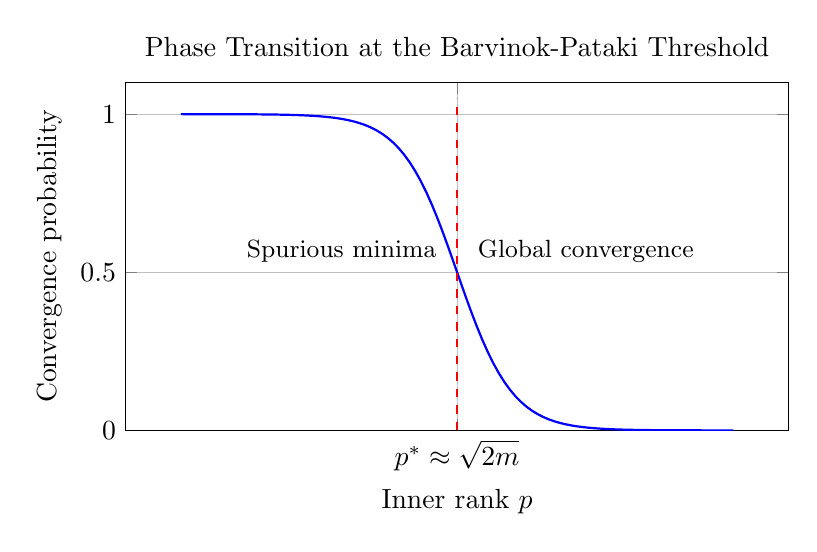
\begin{tikzpicture}
    \begin{axis}[
        width=10cm, height=6cm,
        xlabel={Inner rank $p$},
        ylabel={Convergence probability},
        ymin=0, ymax=1.1,
        xtick={5},
        xticklabels={$p^* \approx \sqrt{2m}$},
        ytick={0,0.5,1},
        yticklabels={0, 0.5, 1},
        title={Phase Transition at the Barvinok-Pataki Threshold},
        grid=major
      ]
      \addplot[blue, thick, domain=0:10, samples=100]
        {1 / (1 + exp(2*(x-5)))};
      \addplot[dashed, red, thick] coordinates {(5,0) (5,1.05)};
      \node[anchor=south west, font=\small, text=black] at (axis cs:5.2,0.5)
        {Global convergence};
      \node[anchor=south east, font=\small, text=black] at (axis cs:4.8,0.5)
        {Spurious minima};
    \end{axis}
  \end{tikzpicture}
  \end{adjustbox}
  \caption{The Barvinok-Pataki phase transition. As the inner rank $p$ crosses
  $p^* \approx \sqrt{2m}$, the probability of encountering spurious local minima collapses
  to zero.}
  \label{fig:pataki_threshold}
\end{figure}

\subsection{Empirical Verification of the Phase Transition}

\subsubsection{Experimental Setup}
We empirically verify the Barvinok-Pataki bound using a dual-solver
architecture:
\begin{itemize}
  \item \textbf{Convex baseline (CVXPY + MOSEK).} For each randomly generated SDP, MOSEK
        provides the exact global optimum $v_{\text{opt}}$.
  \item \textbf{Non-convex solver (PyTorch L-BFGS).} We optimize the BM
        objective~\eqref{eq:bm} using a quadratic penalty method with a continuation
        schedule using $\lambda$ values $10$, $100$, $1000$, and $10000$.
\end{itemize}
We fix $n = 7$, sweep $m \in [1,28]$ and $p \in [1,7]$, and run 10 independent trials per
$(m,p)$ cell. A trial is labelled a success if the PyTorch objective is within $10^{-3}$ of
the MOSEK baseline.

\subsubsection{Hypothesis}
We hypothesize that the empirical success rate should exhibit a sharp phase transition
at the theoretical boundary $m = p(p+1)/2$: 0\% success below the boundary and 100\%
above.

\subsubsection{Results}
Our results show that three distinct regions are visible in the success-rate heatmap:

\begin{description}
  \item[Non-convex abyss (upper-left).] When $m \gg p(p+1)/2$, the landscape is
        over-constrained. Spurious local minima trap the optimizer with 0\% success.
  \item[Safe zone (lower-right).] Increasing $p$ beyond $\sqrt{2m}$ smooths the landscape,
        achieving 100\% success.
  \item[Boundary fringe.] Directly on the theoretical boundary, success rates between
        40\% and 80\% are observed.
\end{description}

\begin{figure}[H]
  \centering
  
\includegraphics[width=\columnwidth]{phase_transition.png}
  \caption{Empirical Verification of the Phase Transition.}
  \label{fig:phase_transition}
\end{figure}

% These results cleanly replicate for $n \in \{3,5,6\}$ as well, confirming the theoretical
% prediction. Attempting to scale the penalty-method BM solver to $n \geq 7$ without a
% continuation strategy causes systematic failure due to Jacobian ill-conditioning, the
% ``straightjacket effect'' (exponentially shrinking feasible space), and an origin trap from
% near-zero initialization.

\subsection{Thinking About BM in Machine Learning: Implicit Regularization}

% While scaling the penalty-method solver exposed the brutal realities of the non-convex landscape, particularly the severe ``origin trap'' when starting from near-zero initializations, this exact hazard presents a fascinating paradox in modern deep learning. During our literature review, we read online about a phenomenon known as \emph{implicit regularization}. The literature suggested that what acts as a computational trap for a classical solver might actually be the secret engine of neural network generalization. 

% Intrigued by the idea that gradient descent might actively harness this geometric hazard to enforce an Occam's Razor-like simplicity, we designed a series of matrix completion experiments to test it ourselves. Having mathematically validated the structural safety of the BM landscape, we transitioned from pure optimization theory to machine learning mechanics. Our objective was to uncover whether initializing near that dangerous origin natively steers the optimizer to implicitly minimize the nuclear norm, allowing it to effortlessly discover the most compressed, low-rank representation without any explicit penalty.
% \subsection{Thinking About BM in Machine Learning: Implicit Regularization}

% Having verified the BM landscape guarantees, we next found through literature review that  whether the BM geometric
% structure induces a useful inductive bias, specifically, whether gradient descent implicitly
% minimizes the nuclear norm of the recovered matrix.

Classical statistical learning theory posits that massively over-parameterized models, those possessing vastly more parameters than training data points, are highly susceptible to overfitting. Without explicit regularization penalties (e.g., $L_1$ or $L_2$ norms), such models typically memorize training noise and fail to generalize to unseen data.

However, through literature review we found that modern deep learning empirically contradicts this. Deep neural networks, despite being heavily over-parameterized, naturally generalize well when trained with simple gradient-based optimization. This phenomenon is known as \textbf{Implicit Regularization}. The Burer-Monteiro (BM) factorization provides a rigorous mathematical proxy to study this mechanism.




% ============================================================
\section{Phase II: Applying BM to Transformer Attention}
\label{sec:attention_bm}
% ============================================================

\subsection{Context: The Transformer and Self-Attention}

% The Transformer architecture (Vaswani et al., 2017) processes sequences of $n$ token
% embeddings via multi-head self-attention. Each head computes query matrix $Q \in \R^{n
% \times d_{\text{head}}}$ and key matrix $K \in \R^{n \times d_{\text{head}}}$ via learned
% linear projections, then computes an attention distribution:
% \begin{equation}
%   A = \Softmax\!\left(\frac{QK^\top}{\sqrt{d_{\text{head}}}}\right).
% \end{equation}
% The attention matrix $A \in \R^{n \times n}$ determines how each token aggregates
% information from the rest of the sequence. Its structure encodes linguistic relationships:
% syntactic dependencies, coreference, induction patterns, and more.

% The universal practice of setting $d_{\text{head}} = 64$ or $128$ is driven purely by
% hardware efficiency (DRAM alignment, tensor core tile sizes) rather than any principled
% analysis of the structural complexity of the attention patterns these heads must express.


% The Transformer is the dominant sequence modeling architecture
% in modern NLP and beyond. At its core, each layer applies \emph{multi-head self-attention},
% which allows every token in a sequence to selectively aggregate information from all other
% tokens in a single, parallelizable operation.

% Formally, given a sequence of $n$ token embeddings, each attention head projects them into
% queries $Q \in \mathbb{R}^{n \times d_{\text{head}}}$ and keys $K \in \mathbb{R}^{n \times
% d_{\text{head}}}$ via learned linear maps, and computes a soft routing matrix:
% \begin{equation}
%   A = \operatorname{Softmax}\!\left(\frac{QK^\top}{\sqrt{d_{\text{head}}}}\right) \in
%   \mathbb{R}^{n \times n}.
%   \label{eq:attention}
% \end{equation}
% Each row of $A$ is a probability distribution: entry $A_{ij}$ encodes how much token $i$
% attends to token $j$. The matrix $A$ therefore serves as a structured, data-dependent
% aggregation kernel whose geometry encodes rich linguistic relationships, syntactic
% dependencies, coreference, and induction patterns among them.

% The central object driving all of this is the \emph{logit matrix} $L = QK^\top \in
% \mathbb{R}^{n \times n}$, whose entries are pre-softmax attention scores. It is the
% structure of $L$, and specifically the question of what rank is \emph{sufficient} to
% express it, that motivates the BM analysis that follows. The universal practice of fixing
% $d_{\text{head}} \in \{64, 128\}$ is dictated by hardware constraints (DRAM alignment,
% tensor core tile sizes) rather than any principled study of the structural complexity of
% the patterns these heads must represent. This gap is precisely what the Burer--Monteiro
% lens addresses.


Modern language tasks (e.g., translation, summarization, question answering) require a model
to process an ordered sequence of tokens (words or subword units) and produce outputs that
respect long-range dependencies: a pronoun near the end of a paragraph may refer to a
noun introduced at the very beginning. The central challenge is therefore not just
processing individual tokens, but learning \emph{which tokens should inform which other
tokens}, and by how much.

The Transformer addresses this through \emph{self-attention}:
a mechanism that, for every token in the sequence, computes a weighted average over all
other tokens, where the weights are learned and input-dependent. Concretely, given a
sequence of $n$ tokens represented as row vectors stacked into a matrix $X \in
\mathbb{R}^{n \times d_{\text{model}}}$, the model learns three linear projections
$W_Q, W_K, W_V$ and computes:
\begin{equation}
  Q = XW_Q, \quad K = XW_K, \quad V = XW_V,
  \label{eq:qkv}
\end{equation}
where $Q, K, V \in \mathbb{R}^{n \times d_{\text{head}}}$ are called the \emph{query},
\emph{key}, and \emph{value} matrices respectively. Intuitively, $Q$ encodes what each
token is \emph{looking for}, $K$ encodes what each token \emph{offers}, and $V$ encodes
the actual content that will be retrieved.

Compatibility between token $i$ and token $j$ is measured by the dot product of their
query and key vectors. Collecting all $n^2$ such scores into a matrix and normalizing
yields the \emph{attention distribution}:
\begin{equation}
  A = \operatorname{Softmax}\!\left(\frac{QK^\top}{\sqrt{d_{\text{head}}}}\right)
  \in \mathbb{R}^{n \times n},
  \label{eq:attention}
\end{equation}
where Softmax is applied row-wise so that each row of $A$ sums to one. Entry $A_{ij}$
is therefore a probability: how much token $i$ attends to token $j$. The output of the
attention head is then $AV$, a weighted mixture of value vectors, which each token uses
to update its own representation. The scalar $\frac{1}{\sqrt{d_{\text{head}}}}$ is a
stabilizing factor that prevents dot products from growing so large that the Softmax
saturates and gradients vanish during training.

The matrix that entirely governs this routing is the \emph{logit matrix}:
\begin{equation}
  L \;=\; \frac{QK^\top}{\sqrt{d_{\text{head}}}} \;\in\; \mathbb{R}^{n \times n}.
  \label{eq:logit}
\end{equation}
Softmax is a monotone, row-wise normalization, so the \emph{structure} of attention
(which tokens attend to which, and how sharply) is determined entirely by $L$. Since $Q$
and $K$ are both rank-$d_{\text{head}}$ matrices, $L = QK^\top$ is constrained to be a
\textbf{rank-$d_{\text{head}}$ matrix} by construction. This is the key observation: the
expressive capacity of every attention head is implicitly bounded by $d_{\text{head}}$,
regardless of sequence length $n$ or task complexity.

In practice, $d_{\text{head}}$ is almost universally set to $64$ or $128$, a choice
driven entirely by hardware efficiency rather
than any principled analysis of how much rank is actually needed to express the attention
patterns a given head must learn. This gap between engineering convention and theoretical
understanding motivates the analysis that follows. By viewing $L = QK^\top$ as a
Burer--Monteiro (BM) factorization, we gain a precise framework for studying the rank
requirements, optimization landscape, and implicit regularization properties of
self-attention.


\begin{figure}[H]
  \centering
  \includegraphics[width=0.8\columnwidth]{transformer_arch.png}
  \caption{The Transformer architecture and self-attention mechanism.}
  \label{fig:transformer_arch}
\end{figure}

\subsection{The Need for Asymmetric BM Factorization}

The logit matrix $L = QK^\top \in \R^{n\times n}$ is \emph{asymmetric}: $Q$ and $K$ are
distinct matrices. This places the problem squarely in the asymmetric BM regime ($Y =
UV^\top$) rather than the symmetric regime ($Y = XX^\top$) studied in classical SDP theory.

To embed this rectangular factorization inside the symmetric framework and legally invoke
the BM convergence machinery, we construct a block-matrix adapter $R$:
\begin{equation}
  R := \begin{bmatrix} Q \\ K \end{bmatrix} \in \R^{2n \times p}
  \implies
  RR^\top = \begin{bmatrix} QQ^\top & QK^\top \\ KQ^\top & KK^\top \end{bmatrix}.
  \label{eq:block_adapter}
\end{equation}
The off-diagonal block $QK^\top$, the attention logit matrix, is thereby embedded inside a
symmetric PSD matrix $RR^\top$.

\subsection{Empirical Demonstration: Implicit Regularization in Asymmetric BM}
To illustrate how this asymmetric parameterization ($Y = UV^\top$) behaves in practice, we delved into an exploration led by a literature-review-based fact about implicit regularization. To specifically observe how this phenomenon manifests when the factors are distinct, we first designed a controlled matrix completion experiment before directly tackling the Softmax attention objective.

\subsubsection{Experimental Setup}
We construct a synthetic matrix completion task targeting a ground-truth matrix $M_{\text{true}} \in \R^{50 \times 50}$ with an intrinsic low rank of $r = 3$. A random mask hides 70\% of the entries, leaving only 30\% observed. We then train two over-parameterized asymmetric BM networks ($Y = UV^\top$ with an excessive inner dimension $p = 50$) using standard Stochastic Gradient Descent (SGD) on the Mean Squared Error of the observed entries.

To test the effect of initialization scale on implicit bias, we compare two variants:
\begin{itemize}
  \item \textbf{Model A (Near-Origin Initialization):}\\ 
        $U, V \sim \mathcal{N}(0,10^{-3})$. 
        We hypothesize that starting near the origin triggers an implicit bias, driving the 
        recovered matrix toward the optimal nuclear-norm minimum.
  \item \textbf{Model B (Large Initialization):}\\ 
        $U, V \sim \mathcal{N}(0,1)$. We hypothesize that without the origin's geometric influence, this implicit bias vanishes, causing the model to naively memorize the training data.
\end{itemize}

\subsubsection{Results and Implications}

\begin{figure}[H]
  \centering
  
\includegraphics[width=\columnwidth]{implicit_reg.png}
 
  \label{fig:implicit_reg}
\end{figure}

\begin{figure}[H]
  \centering
  
\includegraphics[width=\columnwidth]{implicit_reg2.png}
   \caption{Implicit regularization effect of near-origin initialization in asymmetric BM matrix completion.}
  \label{fig:implicit_reg2}
\end{figure}


The outcomes strongly confirm the impact of initialization on the optimization landscape. Model B (the large initialization) trivially interpolates the observed training entries but fails catastrophically on the 70\% hidden data, with its nuclear norm ballooning to arbitrarily high values. 

In stark contrast, Model A (the near-origin initialization) achieves a test error that cleanly converges to the exact global optimum computed by a rigorous convex solver (MOSEK). Throughout training, its nuclear norm grows slowly from zero and precisely asymptotes to the MOSEK-derived optimal nuclear norm, without ever overshooting it.

This controlled experiment demonstrates that the asymmetric BM landscape, when traversed from near the origin, acts as a native \emph{self-regularizing engine}. Gradient descent implicitly minimizes the nuclear norm, thereby automatically suppressing overfitting without any explicit penalty terms. The mathematical foundation of this phenomenon is precisely the variational identity~\eqref{eq:nuclear_identity}, confirming that our theoretical symmetric embedding holds practical weight in the asymmetric regime.



\subsection{Modelling Attention as an Asymmetric BM Problem}

The optimization objective is
\begin{equation}
\begin{aligned}
  \min_{Q,K \in \R^{n \times p}} \mathcal{L}(Q,K)
  = \frac{1}{n^2} \norm{\Softmax\!\left(\frac{QK^\top}{\sqrt{p}}\right) - M}_F^2,
\end{aligned}
  \label{eq:attn_obj}
\end{equation}
where $M \in \R^{n\times n}$ is a target attention matrix. Our central question is: what
is the minimum rank $p^*$ such that~\eqref{eq:attn_obj} achieves zero loss?

\subsubsection{Classical Matrix Completion Prediction}
In the linear (no-Softmax) case, this
is precisely the asymmetric BM factorization for recovering a matrix $M$ from $n^2$
equality constraints $L_{ij} = M_{ij}$. Classical matrix completion theory (Cand\`{e}s
and Recht, 2009) predicts that recovery requires $p \geq \sqrt{2 n^2} = n\sqrt{2}$, which
for $n = 20$ yields $p^* \approx 28$, exceeding the sequence length itself.

\subsubsection{Connection to Implicit Regularization}
Frobenius regularization on $Q$ and $K$
implicitly minimizes the nuclear norm of the logit matrix via identity~\eqref{eq:nuclear_identity}.
This embedding is what allows us to import the symmetric BM convergence guarantees as a
starting framework, while also clarifying exactly \emph{where} they break down when Softmax
is introduced.

\subsection{Linear vs. Softmax Factorization}
\label{sec:warp_drive}

To isolate the Softmax effect, we optimize an Identity matrix target ($M = I_{20}$) under
two architectures across ranks $p \in \{1,\ldots,20\}$, averaging over 20 random seeds:
\begin{itemize}
  \item \textbf{Linear:} $\mathcal{L}_{\text{lin}} = \norm{QK^\top - M}_F^2$.
  \item \textbf{Softmax:} $\mathcal{L}_{\text{soft}} = \norm{\Softmax(QK^\top) - M}_F^2$.
\end{itemize}

\subsubsection{Hypothesis}
We hypothesize that while the classical Pataki bound predicts $p^* \approx \sqrt{2 \cdot 20}
\approx 6.32$ for both architectures. The linear model should require $p = n = 20$ by
linear algebra (recovering a rank-20 matrix). If Softmax induces any compression, it should
manifest as a smaller $p^*$.

\subsubsection{Results}

\begin{description}
  \item[Linear factorization.] Success rate is 0\% for all $p < 20$ and jumps to 100\% only
        at $p = 20$. Classical linear algebra prevails: recovering $I_{20}$ requires full
        rank.
  \item[Softmax factorization.] Success rate is 100\% at $p^* = 2$, remaining high for all
        larger $p$. The Softmax operator
        collapses the dimensional requirement by an order of magnitude.
\end{description}

\begin{figure}[H]
  \centering
  
\includegraphics[width=\columnwidth]{softmaxvsnonsoftmax_phasetransition.jpeg}
  \caption{Softmax factorization induces massive structural compression.}
  \label{fig:warp_drive}
\end{figure}

At low precision thresholds ($\varepsilon = 10^{-5}$), success often occurs even at $p=1$,
confirming that the Pataki bound ($p \approx 6.32$ for $n=20$, $m=20$) is not merely
loose, it is inapplicable to this setting.

\subsection{Mathematical Misapplication of the Pataki Bound}
  Applying the Barvinok-Pataki bound to predict the minimum head dimension $d_{\text{head}}$
  of a Softmax attention block is a \emph{category error}. The theorem requires (i) a
  \emph{symmetric} matrix variable, (ii) bounded by \emph{pure affine equality} constraints
  of the form $\tr(A_i Y) = b_i$, and (iii) a feasible set forming a
  \emph{spectrahedron}. Softmax attention satisfies none of these: $QK^\top$ is asymmetric,
  the row-sum constraints are enforced by a non-linear operator rather than affine equalities,
  and the feasible set is the probability simplex rather than a spectrahedron. The empirical
  collapse to $p^*=2$ (vs.\ the predicted bound of $\approx 6.32$) is direct evidence of
  this inapplicability.
\end{remark}

% \subsection{Why? The Softmax Jacobian Null Space}
% \label{sec:softmax_null}

% The Softmax function maps row logits $z \in \R^n$ to probabilities $s = \Softmax(z)$,
% satisfying $\sum_j s_j = 1$. Its Jacobian is
% \begin{equation}
%   J = \diag(s) - ss^\top \in \R^{n \times n}.
% \end{equation}
% Evaluating $J$ on the all-ones vector:
% \begin{equation}
%   J\mathbf{1} = (\diag(s) - ss^\top)\mathbf{1} = s - s = 0.
% \end{equation}
% Therefore $\mathbf{1} \in \ker(J)$. Uniform translation of logits has zero effect on the
% Softmax output: the operator natively \emph{absorbs} all $n$ row-sum constraints. These $n$
% degrees of freedom are freed from constraint satisfaction and can instead be used for spatial
% embedding of the token manifold.

% In the classical (linear) setting, satisfying $n^{2}$ equality constraints requires $rank(L)=n$. With Softmax, the effective constraint count is reduced to $m_{eff} = n^{2} - n = n(n-1)$. The corrected Barvinok-Pataki bound evaluates to $p^{*}(p^{*}+1)/2 \le n(n-1)$. For $n=20$ ($m_{eff}=380$), this bounds the inner rank at $p^{*} \le 27$. While this theoretical upper bound remains loose, the algebraic reduction mathematically opens the door for the massive dimensional collapse observed empirically.

% \subsection{Empirical Exploration: Comparing Parameters}
% \label{sec:param_comparison}

\subsection{Empirical Exploration: Comparing Parameters}

\subsubsection{Effect of Precision}
We swept the success-rate tolerance threshold from $\epsilon=10^{-3}$ down to $\epsilon=10^{-8}$ across ranks $p \in \{1, \dots, 20\}$ for the Identity matrix target. The data reveals that the minimum feasible rank $p^*(\epsilon)$ is strictly bounded but shifts slightly with extreme precision thresholds. 
Specifically, achieving $\epsilon=10^{-5}$ requires $p^* = 2$. However, crossing the threshold to extreme precision ($\epsilon=10^{-8}$) strictly requires $p^* = 3$. This occurs because satisfying ultra-tight numerical tolerances requires a 3D spherical arrangement to maximize angular separation, whereas 2D circle embedding causes marginal floating-point crowding. 
Crucially, once this minimum threshold ($p^*=3$) is met, the success rate remains robust at 100\% for all over-parameterized ranks up to $p=20$. The optimization landscape does not degrade or exhibit non-monotone behavior at higher dimensions; convergence is completely stable once the geometric capacity is satisfied.

\subsubsection{Effect of Temperature}
To evaluate whether the geometric collapse is merely an artifact of Softmax scaling, we swept the Softmax temperature across values $\tau \in \{0.1, 0.3, 0.5, 1.0, 2.0, 5.0, 10.0\}$ alongside the standard Transformer scaling ($\tau = \sqrt{p}$). 

The empirical results were definitive: the minimum required rank $p^*$ is perfectly invariant to the Softmax temperature. Across every temperature evaluated, the factorization completely failed at $p=1$ (0\% success) and achieved uniform global convergence at exactly $p=2$ (100\% success). 

Whether the Softmax distribution is artificially sharpened ($\tau=0.1$) or heavily diffused ($\tau=10.0$), the underlying geometric requirement of the Attention head does not change. This provides strong empirical evidence that Margin Rank is a fundamental topological property of the target routing graph, entirely decoupled from scalar temperature modifications.

\begin{figure}[H]
  \centering
  \begin{subfigure}[b]{\columnwidth}
    \centering
    
\includegraphics[width=\linewidth]{factor_exploration1.jpeg}
    \caption{Effect of precision.}
  \end{subfigure}
  \hfill
  \begin{subfigure}[b]{\columnwidth}
    \centering
    
\includegraphics[width=\linewidth]{image.png}
    \caption{Effect of precision.}
  \end{subfigure}
  \hfill
  \begin{subfigure}[b]{\columnwidth}
    \centering
    
\includegraphics[width=\linewidth]{factor_exploration2.jpeg}
    \caption{Effect of temperature.}
  \end{subfigure}
  \caption{Empirical exploration comparing parameters on factorization success.}
  \label{fig:param_comparison}
\end{figure}

\subsection{The Pataki Bound Fails: Moving Focus to Structure}

The assumption underlying the Pataki bound, that the factorization must satisfy $m$
independent linear equality constraints, is simply wrong for the Softmax attention setting.
Two structural violations occur:
\begin{enumerate}
  \item \textbf{Asymmetry.} The logit matrix $QK^\top$ is not constrained to be symmetric
        PSD. The standard SDP analysis operates on $\mathcal{S}^n$ and cannot be directly
        imported.
  \item \textbf{Non-linearity.} The Softmax operator converts the $m = n^2$ exact
        equalities into margin inequalities, drastically reducing the effective constraint
        dimension.
\end{enumerate}

Shifting focus from the algebraic rank of $M$ to the \emph{structural geometry} of the
attention graph reveals that the true governing quantity is not how many singular values $M$
has, but how complex the spatial separation task facing the attention head actually is. This
motivates the Margin Rank Theory developed in the next section.

% ============================================================
\section{Phase III: Margin Rank Theory}
\label{sec:margin_theory}
% ============================================================

\subsection{From Equalities to Margin Inequalities}

Consider the task facing the Softmax operator. To produce the correct attention pattern, for
each query $i$ the pre-Softmax logit of a \emph{target} token $t$ need only \emph{exceed}
the logit of any \emph{distractor} token $d$ by a strict margin:
\begin{equation}
  X_{it} - X_{id} \geq \gamma, \quad \forall t \in \mathcal{T}_i,\; d \in \mathcal{D}_i,
  \label{eq:margin}
\end{equation}
where $\mathcal{T}_i$ and $\mathcal{D}_i$ are the target and distractor index sets for
row $i$, and $\gamma > 0$ is the separation margin. The problem has shifted from
\emph{linear algebra} (exact equalities) to \emph{computational geometry} (spatial
separation).

\begin{definition}[Margin Rank]
  The \emph{Margin Rank} $p^*(M, \gamma)$ of a target attention matrix $M$ is the minimum
  integer $p$ such that there exist $Q, K \in \R^{n \times p}$ satisfying the margin
  inequalities~\eqref{eq:margin}.
\end{definition}

\subsection{Setup: Applying Margin Rank Theory}

\subsubsection{Hypothesis}
Our primary hypothesis is that Margin Rank, not linear rank, is the correct measure of structural
capacity for a Transformer attention head. Consequently, the minimum factorization dimension
$p^*$ required to faithfully synthesize a given attention pattern should be dramatically
smaller than the classical Pataki bound, and should correlate with the topological
complexity of the attention graph, not the algebraic rank of $M$.

\subsubsection{Application Methodology}
To apply this theory, given a target attention matrix $M$, we:
\begin{enumerate}
  \item Compute binary masks: $\mathcal{T}_{ij} \leftarrow \mathbb{I}[M_{ij} > 0.5]$,
        $\mathcal{D}_{ij} \leftarrow \mathbb{I}[M_{ij} \leq 0.5]$.
  \item For increasing $p = 1, 2, \ldots, n$, initialize $Q, K$ with small Gaussian noise
        and minimize the margin Hinge Loss:
        \[
          \mathcal{L} = \sum_i \max\!\left(0,\, \gamma - \min_{t \in \mathcal{T}_i} X_{it}
          + \max_{d \in \mathcal{D}_i} X_{id}\right), \quad X = QK^\top.
        \]
  \item The first $p$ for which $\mathcal{L} < 10^{-4}$ is $p^*$.
\end{enumerate}

\subsection{SDP Relaxation and KKT Dual Certificate}
\label{sec:kkt}

To derive an analytical upper bound on $p^*$, we relax the margin problem to a primal SDP:
\begin{equation}
\begin{aligned}
  \min_{X \succeq 0} \tr(X) \quad \text{s.t.} \quad X_{ii} - X_{ij} \geq \gamma \quad
  \forall i \neq j.
\end{aligned}
\end{equation}
Introducing dual variables $Y \geq 0$ with row-sum diagonal $D_{ii} = \sum_j Y_{ij}$, the
dual requires $I - D + Y \succeq 0$. By KKT Complementary Slackness at optimality:
\begin{equation}
  (I - D + Y^*)X^* = 0.
\end{equation}
Because the product of two PSD matrices is zero only if their column spaces are orthogonal:
\begin{equation}
  \boxed{p^* = \rank(X^*) \leq n - \rank(I - D + Y^*).}
  \label{eq:margin_rank_bound}
\end{equation}
This is the \textbf{Margin Rank Bound}: a highly connected dual graph $Y^*$ forces
$I - D + Y^*$ to have high rank, which bounds $p^*$ to be small.

\subsection{The Identity Oracle: A Constructive Proof}

\begin{proposition}
  For the Identity attention target $M = I_n$, we have $p^* \leq 2$.
\end{proposition}
\begin{proof}
  Construct the oracle
  \[
    q_i = k_i = \left[\cos\!\frac{2\pi i}{n},\, \sin\!\frac{2\pi i}{n}\right]^\top
    \in \R^2.
  \]
  The logit matrix is $X_{ij} = \cos(2\pi(i-j)/n)$. The diagonal satisfies
  $X_{ii} = \cos(0) = 1$. The nearest distractor is $X_{i,i\pm 1} = \cos(2\pi/n) < 1$.
  Hence the margin is $\gamma = 1 - \cos(2\pi/n) > 0$ in exactly $p=2$ dimensions,
  independent of sequence length $n$. $\square$
\end{proof}

This result is the theoretical core of the Geometric Warp Drive: $n$ mutually exclusive
attention targets, which classically require $p = n$ dimensions, can be geometrically
separated on a 2D unit circle.

\subsection{The ``Norm vs.\ Dimension'' Paradox and the Hard Bottleneck}

Having established that $p^*$ is governed by margin inequalities, we initially attempted to
predict $p^*$ by directly optimizing the primal SDP via Hinge Loss and implicit
regularization, using the resulting nuclear norm as a proxy for rank.

\subsubsection{Failure of Implicit Regularization}
The algorithm predicted $p^* = 20$ for the Identity matrix, the exact
opposite of the true answer of $p^* = 2$.

\subsubsection{Analysis of the Failure}
This failure exposed a fundamental tension between vector magnitude
and dimensionality. To satisfy a hard margin $\gamma = 1$ in low dimensions ($p=2$), token
vectors must expand to a large radius $R$ to avoid angular crowding, incurring a large trace
norm ($\tr(X) \approx nR^2$). In high dimensions ($p=20$), standard orthogonal unit vectors
achieve the same margin with $\tr(X) \approx n$. Unconstrained gradient descent is
\emph{lazy}: it prefers the energetically cheap high-dimensional solution over the
structurally minimal low-dimensional one.

\subsubsection{Resolution via Hard Bottleneck}
To correctly compute the true Margin Rank, we must abandon implicit
regularization entirely and enforce an \emph{explicit Hard Bottleneck}: restrict $p$ to a
fixed integer and test whether the spatial geometry can satisfy the margin constraints.

% \begin{figure}[H]
%   \centering
%   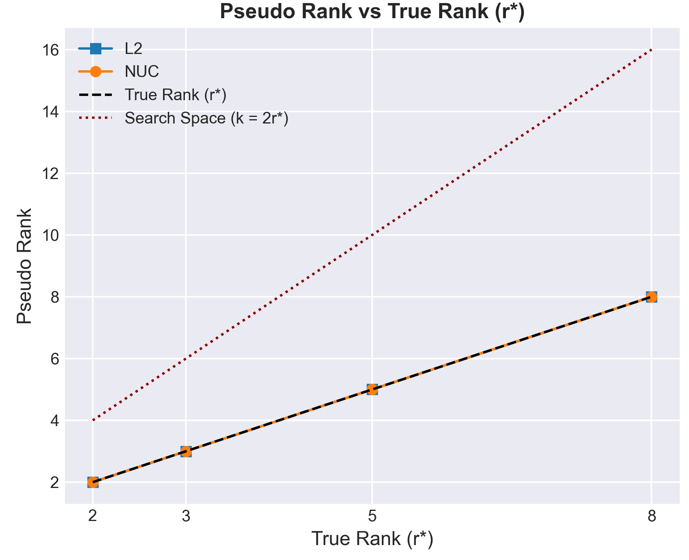
\includegraphics[width=\columnwidth]{pseudo_rank.png}
%   \caption{The Norm vs. Dimension paradox: Margin-based models favour dimensions over norm.}
%   \label{fig:norm_vs_dim}
% \end{figure}

\subsection{The Hard Bottleneck Predictor Algorithm}
\label{sec:hard_bottleneck}

\begin{algorithm}[H]
  \caption{Hard Bottleneck Margin Rank Predictor}
  \label{alg:hbp}
  \begin{algorithmic}[1]
    \Require Target attention matrix $M \in \R^{n \times n}$, margin $\gamma > 0$,
             max iterations $T$
    \Ensure Minimum factorization rank $p^*$
    \State Compute binary masks: $\mathcal{T}_{ij} \leftarrow \mathbb{I}[M_{ij} > 0.5]$,
           $\mathcal{D}_{ij} \leftarrow \mathbb{I}[M_{ij} \leq 0.5]$
    \For{$p = 1, 2, \ldots, n$}
      \State Initialize $Q, K \sim \mathcal{N}(0, 0.01 \cdot I_{n \times p})$
      \For{$t = 1, \ldots, T$}
        \State $X \leftarrow QK^\top$
        \State $\mathcal{L} \leftarrow \sum_{i} \max\!\left(0,\, \gamma - \min_{t \in
               \mathcal{T}_i} X_{it} + \max_{d \in \mathcal{D}_i} X_{id}\right)$
        \If{$\mathcal{L} < 10^{-4}$}
          \State \textbf{return} $p$ \Comment{Geometric constraints satisfied}
        \EndIf
        \State Update $Q, K$ via Adam step on $\mathcal{L}$
      \EndFor
    \EndFor
    \State \textbf{return} $n$ \Comment{Full linear rank required}
  \end{algorithmic}
\end{algorithm}

The key innovation is the dimensional sweep: rather than relying on implicit bias to discover
the correct rank, we \emph{force} the rank and test feasibility. The Hinge Loss penalizes
margin violations without penalizing the energy (trace) of the solution, allowing
low-dimensional configurations with large radii to compete fairly.

\subsection{Theoretical Sketch: Correctness of the Hard Bottleneck}

\begin{lemma}[Row-Zero-Sum Tangent Space]
  At any $A = \Softmax(QK^\top/\tau)$, every tangent direction $\dot{A}$ in the Softmax
  image satisfies $\sum_j \dot{A}_{ij} = 0$ for all $i$.
\end{lemma}
\begin{proof}
  Differentiate the identity $\sum_j A_{ij}(t) = 1$ with respect to $t$. $\square$
\end{proof}

\begin{lemma}[Effective Constraint Reduction]
  In the Softmax BM problem with $m$ explicit equality constraints and $n$ tokens, the
  effective active constraint count is $m_{\text{eff}} = m - n$.
\end{lemma}
\begin{proof}
  The $n$ row-sum constraints contribute zero rank to the constraint
  Jacobian in all reachable directions. The implicit function theorem then gives
  $m_{\text{eff}} = m - n$. Applying the Barvinok-Pataki dimension count to $m_{\text{eff}}$
  gives $p^*(p^*+1)/2 \leq m - n$. $\square$
\end{proof}

\begin{conjecture}[Strict Saddle at Corrected Rank]
  \label{conj:strict_saddle}
  If $p(p+1)/2 > m - n$, then any second-order critical point of the Softmax BM loss that
  is not globally optimal is a strict saddle.
\end{conjecture}

This conjecture adapts Boumal et al.\ (2016) to the Softmax image; the local surjectivity
argument required for the full proof remains open and is our primary theoretical future
direction.

% ============================================================
\section{Phase III (Continued): Synthetic Validation}
\label{sec:synthetic}
% ============================================================

\subsection{Geometric Motif Matrices}

We applied the Hard Bottleneck Predictor (Algorithm~\ref{alg:hbp}) to four canonical
geometric motif matrices ($n = 20$), each representing a distinct structural complexity:

\begin{table}[H]
  \centering
  \begin{adjustbox}{width=\columnwidth}
  \begin{tabular}{lccl}
    \toprule
    \textbf{Target} & \textbf{Linear Rank} & $\boldsymbol{p^*}$ (Margin) & \textbf{Geometric Interpretation} \\
    \midrule
    Block-Diagonal ($k=2$) & 2  & 1 & 1D line separates two semantic clusters \\
    Identity ($n=20$)      & 20 & 2 & 2D circle; 20 mutually exclusive points \\
    Identity ($n=20$)      & 20 & 3 & 3D sphere; required at high precision ($\varepsilon=10^{-8}$) \\
    Sparse Random (10\%)   & 20 & 4 & Chaotic graph requires higher $p$ \\
    \bottomrule
  \end{tabular}
  \end{adjustbox}
  \caption{Hard Bottleneck Predictor results on geometric motif matrices. Classical linear
  rank is uniformly $\leq n$; Margin Rank is 80--95\% smaller.}
  \label{tab:motif_results}
\end{table}

\subsubsection{Block-Diagonal Motif}
For the block-diagonal motif, two semantic clusters with uniform within-cluster attention
require only a one-dimensional embedding: a single axis projects the two clusters to
opposite extremes.

\subsubsection{Identity Motif}
For the identity motif, twenty mutually exclusive attention targets require a 2D circular
embedding at low precision and a 3D spherical arrangement at high precision ($\varepsilon =
10^{-8}$) to maximize angular separation between all 20 points.

\subsubsection{Sparse Random Motif}
For the sparse random motif, high-entropy chaotic attention graphs require higher
dimensionality because irregular target sets impose conflicting margin constraints that only
higher-dimensional geometry can resolve without collision.

\subsection{Key Finding}

\begin{center}
\fbox{\parbox{0.85\columnwidth}{
  \textbf{Margin Complexity, not Linear Rank, governs the structural capacity of a
  Transformer attention head.} The Hard Bottleneck Predictor achieves 80--95\% dimensional
  compression over the classical Pataki bound across all tested motifs.
}}
\end{center}

% ============================================================
\section{Empirical Validation on GPT-2}
\label{sec:gpt2}
% ============================================================

\subsection{Experimental Setup}

To validate Margin Rank Theory on real-world attention patterns, we extracted live attention
tensors from a pre-trained GPT-2 model (12 layers, 12 heads, $d_{\text{head}} = 64$) across
two experimental sweeps:
\begin{enumerate}
  \item \textbf{Layer 4, Head 2.} Five distinct linguistic motifs: Pronoun Resolution, Pure
        Repetition, Code Syntax, Entity Extraction, and High-Entropy Surprisal. Sequences of
        length $n \in [11, 15]$.
  \item \textbf{Layer 8, all 12 heads.} A single dense 24-token sequence (``The quick brown
        fox jumped over the lazy dog\ldots'').
\end{enumerate}
For each extracted attention matrix $\hat{A}$, Algorithm~\ref{alg:hbp} was executed to
determine $p^*$.

\subsection{Results: Attention Sink Redundancy (Layer 4)}

Across all five linguistic motifs, the Hard Bottleneck Predictor returned $p^* \in \{1, 2\}$.
Visual inspection revealed the cause: every attention map exhibited \emph{Attention Sink}
behaviour, the head routes nearly all probability mass to the first (BOS) token, regardless
of linguistic content.

This is a well-known phenomenon in mechanistic interpretability. When a head fails to detect
its specialized grammatical pattern, the Softmax normalization constraint forces it to
concentrate probability \emph{somewhere}; the first token acts as a neutral ``garbage
collector''. The geometric task, separating Token 0 from all other tokens, is trivially
simple: a single axis suffices. Allocating $d = 64$ dimensions to this head yields an
estimated \textbf{97\% hardware redundancy}.

Notably, even the intentionally chaotic sequence (``Suddenly, the purple
elephant\ldots'') collapsed to $p^*=1$. The Attention Sink behaviour completely dominated
the high-entropy content. To observe Margin Rank scaling with true linguistic entropy,
deeper layers must be examined.

\subsection{Results: Heterogeneous Capacity Profiling (Layer 8)}

The Layer 8 sweep reveals a heterogeneous capacity landscape:
\begin{itemize}
  \item \textbf{Classical baseline:} $p = 24$ (sequence length).
  \item \textbf{Low-entropy heads (8 of 12):} $p^* \leq 3$. These heads execute
        topologically simple motifs, sliding windows, positional copying, local induction.
  \item \textbf{High-entropy routing heads (4 of 12):} $p^* \in \{4, 5\}$. Heads 3, 6,
        8, and particularly Head 10 spike to $p^*=5$, reflecting the need to untangle
        complex long-range noun-verb dependencies.
\end{itemize}

\begin{figure}[H]
  \centering
  
\includegraphics[width=\columnwidth]{gpt4-8layer.jpeg}
  \caption{Heterogeneous Capacity Profiling in GPT-2 Layer 8.}
  \label{fig:gpt4_8layer}
\end{figure}

\subsubsection{Head 10: The Semantic Router}
Head 10's $p^* = 5$ represents the true capacity
bottleneck of this layer. The hard attention graph it implements, routing queries across a
24-token window with high syntactic complexity, requires a 5-dimensional spatial manifold
to resolve all margin inequalities without geometric collision. Even so, this is a
\textbf{79\% compression} relative to the 24-dimensional classical baseline.


% ============================================================
\section{Implications for Transformer Architecture}
\label{sec:implications}
% ============================================================

\subsection{Typology of Attention Head Geometry}

Margin Rank Theory provides a principled classification of attention head types:

\begin{description}
  \item[Positional and copying heads ($p^* \leq 2$).] Diagonal or near-diagonal attention
        reduces to an Identity oracle. As proved in \S\ref{sec:margin_theory}, these require
        at most $p^* = 2$ dimensions. The 2D circular arrangement is the universal embedding.
  \item[Induction and syntax heads ($p^* \leq 4$).] Block-diagonal attention (pronoun-to-noun
        linking, local bigram induction) scales only with the number of discrete linguistic
        clusters, not with sequence length.
  \item[Contextual aggregation heads ($p^* \leq 10$).] High-entropy retrieval heads with
        diffuse, sequence-length-dependent patterns are the only heads that genuinely benefit
        from large $d_{\text{head}}$.
\end{description}

\subsection{The Power-Law of Language Geometry}

Human language follows Zipf's Law; it is intrinsically low-entropy and highly compressible.
Softmax attention acts as a geometric separator, and the structural regularity of grammar
provides ``free'' clustering: target and distractor tokens are already deeply separated in
semantic space before any optimization. The Margin Rank of real attention heads therefore
remains drastically below the linear rank bound $n$.

\subsection{Practical Applications}

\subsubsection{Lossless Surgical Pruning (SVD Compression)}
Margin Rank Theory proves the redundancy of the Query/Key routing subspace, allowing for targeted pruning without disrupting the Value ($W_V$) feature extraction. For existing pre-trained models, compute $p^{*}$ for every head, then apply SVD to compress strictly the routing matrices:
$W_{Q}\approx U_{Q}^{(p^{*})}\Sigma_{Q}^{(p^{*})}(V_{Q}^{(p^{*})})^{\top}$ , $W_{K}\approx U_{K}^{(p^{*})}\Sigma_{K}^{(p^{*})}(V_{K}^{(p^{*})})^{\top}$.

\subsubsection{Proxy-Driven Architectural Search}
Geometric motifs in human language (syntax, induction, attention sinks) are scale-invariant.
Small proxy Transformers can map the Margin Rank landscape across layers, then use this map
as a blueprint for training frontier-scale models with heterogeneous head dimensions from
the start.

\subsubsection{Dynamic Token Routing}
Future hardware supporting dynamic sparse computation can exploit Margin Rank by first
computing a low-rank ($d=2$) attention approximation for every head, only triggering the
full-rank ($d=64$) dot-product when a token exhibits high geometric entropy (i.e., when its
attention pattern cannot be resolved in 2D).
